\chapter{Object Localization}
Object localization is the process of finding the position of the object in the satellite image. This process produces a set of candidate windows from the input satellite image which might contain the object. An example of object localization is shown in figure \ref{fig1}

\begin{figure}[!htbp]
\centerline{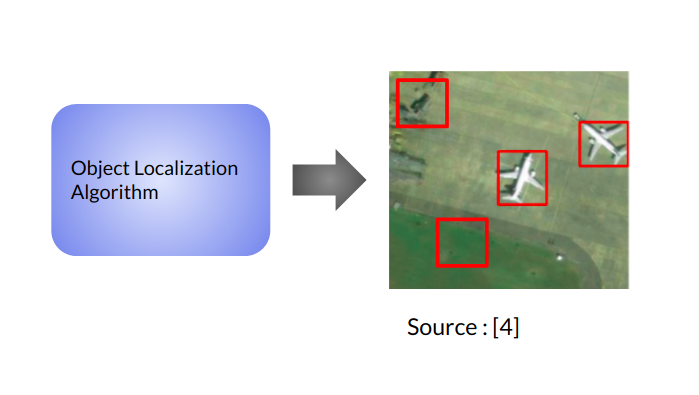
\includegraphics[height=50mm,width=92mm]{img/fig1.png}}
\caption{Example of object localization}
\label{fig1}
\end{figure}

The red colored bounding boxes are the potential object proposals. These bounding boxes will be used for fetaure extraction.

\section{Sliding Window Approach}
Sliding window technique is one of the traditional approach for object localization. In this technique, we define a window of certain height and width which will be sliding throughout the image with a certain stride length. Each of these windows will be provided to the feature extraction module and based on the features it will be classified as object window or non-object window. Working of this approach is described in figure \ref{fig2}. In figure \ref{fig2} each block is a window and the stride length of sliding is 1.

\begin{figure}[!htbp]
\centerline{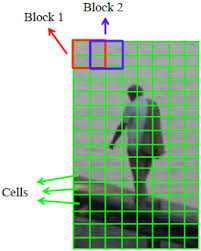
\includegraphics[height=50mm,width=50mm]{img/fig2.jpeg}}
\caption{Sliding window approach, source: https://stackoverflow.com}
\label{fig2}
\end{figure}



\par This approach has many drawbacks, such as it is computationally intensive and the window might not contain the whole object etc. 


\section{Ellipse and Line Segment Detector (ELSD)}
ELSD \cite{b4} can detect rectangular and curved region in an image. It is can be used on any gray-scale images without performing any edge-detection algorithm on the image. It acts as a geometric shape detector. It is used for candidate selection in satellite images because many times the object of interest is circular or ellipsoidal in shape, e.g, wells, oil-tanks etc. ELSD can be carried out in two steps: 
\begin{itemize}
    \item \textbf{Candidate selection: }This is done by performing the process of region growing. Here, we start from a seed pixel and then pixels were grouped into connected regions based on their gradient orientation. The gradient of a pixel can be defined as the direction of change of intensity in the image. 
    \par By region growing and region chaining operation we can get chains of rectangular regions. Now, there are two constraints that will enforce the chain of rectangular regions to be \textit{convex} and \textit{roughly smooth}.
    \par First one is \textbf{convexity constraint}. In this constraint two consecutive rectangular regions should have same directional change in gradient, i.e, $\Delta \theta_i$ and $\Delta \theta_{i+1}$ should have the same sign, given in figure \ref{fig3}.
    \par Second one is the \textbf{roughly smooth constraint}. That is, the change in gradient in two consecutive rectangular region should not exceed the value of $\pi / 2$. This curve growing procedure produce a ``polygonal approximation" \cite{b4} like circular and elliptical shapes. Hence, at the end of this step we get three types of candidates: i) rectangular regions, ii) circular regions and iii) elliptical regions. 
    
    \begin{figure}[!htbp]
    \centerline{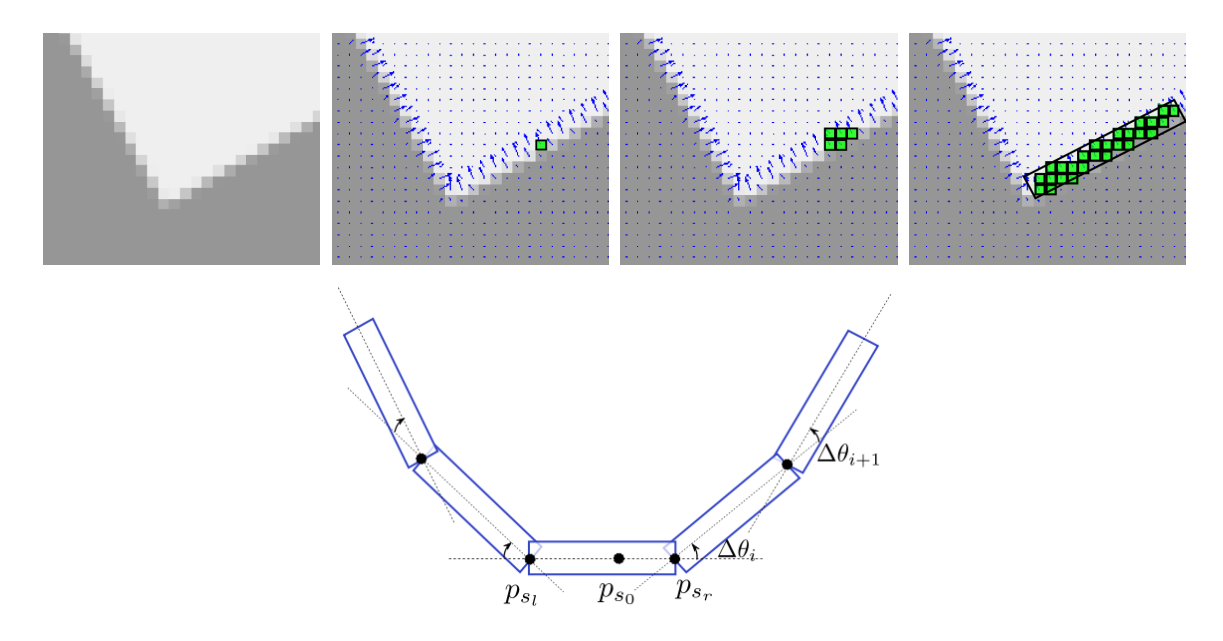
\includegraphics[height=90mm,width=150mm]{img/fig3.png}}
    \caption{Region growing and curve growing. Source: \cite{b4}}
    \label{fig3}
    \end{figure}
    
    \item \textbf{Validation: }It is the process in which we validate the candidates, i.e, it is checked that the candidates have elliptical, circular shape or not. Here, we calculate the number of aligned pixels for each region. The criteria for alignment of a pixel in a curved region is given as: $$Angle(\Delta x(p),\ dir_{\perp}(tan_c(p))\leq \sigma \pi$$ where $\Delta x(p)$ is the gradient of the image $x$ at pixel $p$ and $dir_{\perp}(tan_c(p))$ is the direction orthogonal to the tangent $tan_c(p)$ of the circle or ellipse $c$ at pixel $p$. Here $\sigma$ is the precision value and generally it is set as $1/8$. Some examples of aligned pixels is given in figure \ref{fig4}.
    
    \begin{figure}[!htbp]
    \centerline{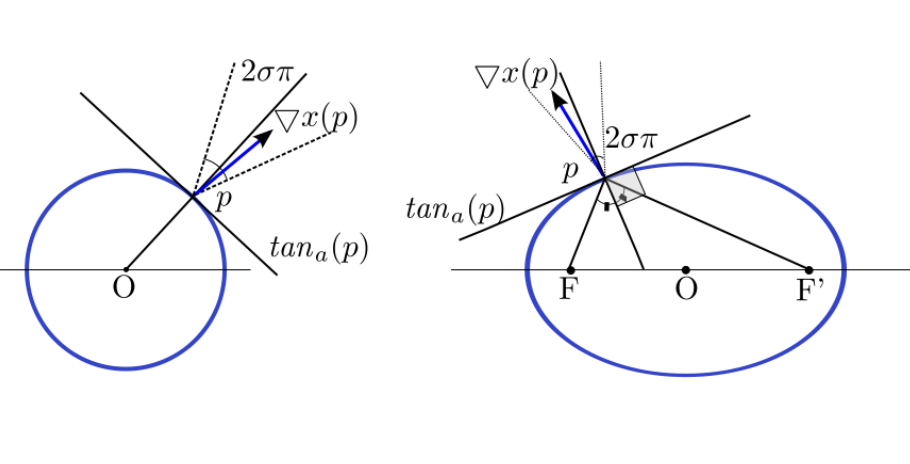
\includegraphics[height=50mm,width=90mm]{img/fig4.png}}
    \caption{``Segments $s$ containing $\sigma$-aligned pixels". Source: \cite{b4}}
    \label{fig4}
    \end{figure}
    
    If the number of aligned pixel for the candidate is greater than a threshold then it is validated as a circular or elliptical shaped region. 
    
\end{itemize}

\par ELSD produces all the elliptical and circular connected regions as output but these regions might not contain our object of interest. Especially, if the object is not circular in shape, e.g, air-crafts. 

\subsection{Modified ELSD}
Zhang et. al. \cite{b6} has modified the traditional ELSD algorithm, specifically for oil-tank detection purpose. As we know that oil-tanks are generally circular in shape and they can not have more radius than a threshold. Hence, alongwith number of aligned pixels constraint they have used another constraint as described below: $$| \sqrt{(cir_r-cen_r)^2+(cir_c-cen_c)^2}-R|\leq \eta,\ and\ \eta \geq 0$$
where $cir_r$ and $cir_c$ are the row and column position of the pixel on the circle respectively and $cen_r$ and $cen_c$ are the row and column position of the center of the circle respectively. $R$ is the radius of the circle and $\eta$ is the threshold for controlling the size of the circular region. Based on these two constraints the candidate regions have been proposed.


\section{Binarized Normed Gradients (BING)}
BING \cite{b2} is an algorithm which can produce potential object windows from an image. It calculates the objectness score for each window and based on that it selects some of the windows if they are above a threshold value. Cheng et. al. \cite{b2} observed that the small image windows of fixed size within an object shares a significant correlation with each other. Thus each image window is re-sized to a fixed size (e.g, $8\times 8$) window. For objectness score calculation, the norm of gradients of each pixel in the $8\times 8$ window is calculated and represented as a 64-dimensional feature vector which will be provided to a cascaded SVM classifier for classification. This 64D feature vector is called normed gradients (NG) feature. If this 64-dimensional feature vector is calculated for binarized version of $8\times 8$ window then this feature will be called binarized normed gradient (BING) feature. 
\par A fixed size window is scanned over the image to find any generic object that are present in it. Each such window will get a score, which will be calculated as: 
$$s_l=W\cdot g_l,\ l=(i,x,y)$$ where $s_l$ is the filter score, $g_l$ is the normed gradient feature, $l$ is the location, $i$ is the size, $W\in \R^{64}$ is the weight vector that has been assigned as co-efficient of filter score for each window, $W$ is learned by a linear SVM model and $(x,y)$ is the position of the window. For each i, a small number of proposals will be selected using non-max suppression. Non-max suppression is an algorithm which eliminates the similar bounding boxes or windows based on a threshold value of overlapping between two windows. Based on the filter score $s_l$, the actual objectness score is calculated using the formula $$o_l=v_i\cdot s_l+t_i$$ where $o_l$ is the objectness score of the window at location $l$, $v_i,\ t_i$ are the co-efficient and a bias term which can be learned with an SVM classifier respectively. Normed gradient features of some object windows and non-object windows are used as ground truth positive and negative samples respectively for training.  

\par Wu et.al. \cite{b5} has used this objectness score to detect potential windows containing air-craft. They have imposed some constraints on the output windows for filtering. The constraints are: 
\begin{itemize}
    \item Windows with high height/width ratio has been chosen where ratio is $$ratio=\frac{max(height, width)}{min(height,width)}$$. If the ratio is above a certain threshold then the window is chosen.
    
    \item Windows, that has area under a certain range $[A_i,A_j]$ is chosen where area of the window is calculated as $$area=height\times width$$.
    
    \item Windows that has objectness score $o_l$ which is above a threshold  value $o_t$ is chosen.
\end{itemize}
\par The result of applying BING on satellite images containing air-crafts is given in figure \ref{fig5}.

\begin{figure}[!htbp]
\centerline{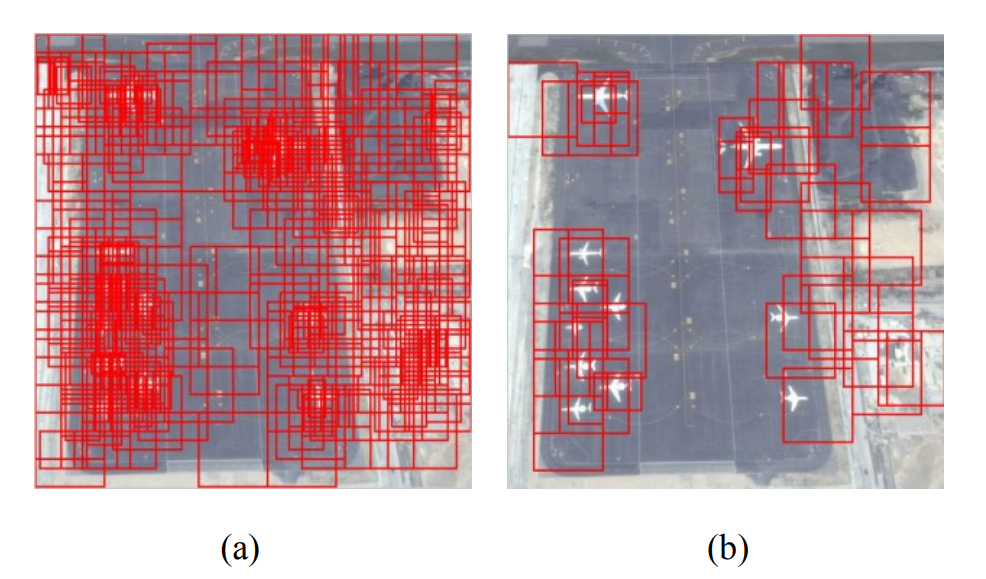
\includegraphics[height=60mm,width=100mm]{img/fig5.png}}
\caption{(a) Bounding boxes proposed by BING. (b) Bounding boxes after imposing the constraints. Source: \cite{b5}}
\label{fig5}
\end{figure}
